% !TEX TS-program = xelatex
% !TEX encoding = UTF-8 Unicode

% Spring 2020 - Summer 2020 - Fall 2020 - Fall 2021
% Tristan Hill, May 07, 2020 - June 12, 2020 - July 08, 2020
% Module Y - Sensors
% Topic 1 - Various Sensors (need new title)

\documentclass[fleqn]{beamer} % for presentation (has nav buttons at bottom)

\usepackage{/home/thill/Documents/lectures/measurements_lectures/measurements_lectures}

\author{ME3023 - Measurements in Mechanical Systems} 

\newcommand{\MNUM}{5\hspace{2mm}} % Module number
\newcommand{\TNUM}{\hspace{2mm}} % Topic number 
\newcommand{\moduletitle}{Sensors}
\newcommand{\topictitle}{Introduction and Overview} 

\newcommand{\sectiontitleI}{Classification of Sensors}
\newcommand{\sectiontitleII}{Analog and Digital Sensors}
\newcommand{\sectiontitleIII}{Example 1: Distance or Range}
\newcommand{\sectiontitleIV}{Example 2: Motion}
\newcommand{\sectiontitleV}{Example 3: Orientation}

\newcommand{\btVFill}{\vskip0pt plus 1filll}

% custom box
\newsavebox{\mybox}

\title{Lecture Module - \moduletitle}

\date{Mechanical Engineering\vspc Tennessee Technological University}

\begin{document}
	
	\lstset{language=MATLAB,basicstyle=\ttfamily\small,showstringspaces=false}
	
	\frame{\titlepage \center\begin{framed}\Large \textbf{Topic \TNUM - \topictitle}\end{framed} \vspace{5mm}}
	
	% Section 0: Outline
	\frame{
		\large \textbf{Topic \TNUM - \topictitle} \vspace{3mm}\\
		
		\begin{itemize}
			
			\item \sectiontitleI    \vspc % Section I
			\item \sectiontitleII 	\vspc % Section II
			\item \sectiontitleIII 	\vspc %Section III
			\item \sectiontitleIV 	\vspc %Section IV
			
		\end{itemize}
		
	}

\section{\sectiontitleI}

% Section I - Frame I:
\frame{  \small
	\frametitle{\sectiontitleI}
	
	a {\PR sensor}, a physical element that employs some natural phenomenon... ...to sense the variable being measured
	
	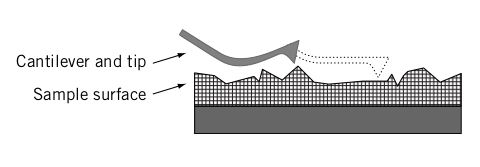
\includegraphics[scale=0.30]{sensor_stage.png}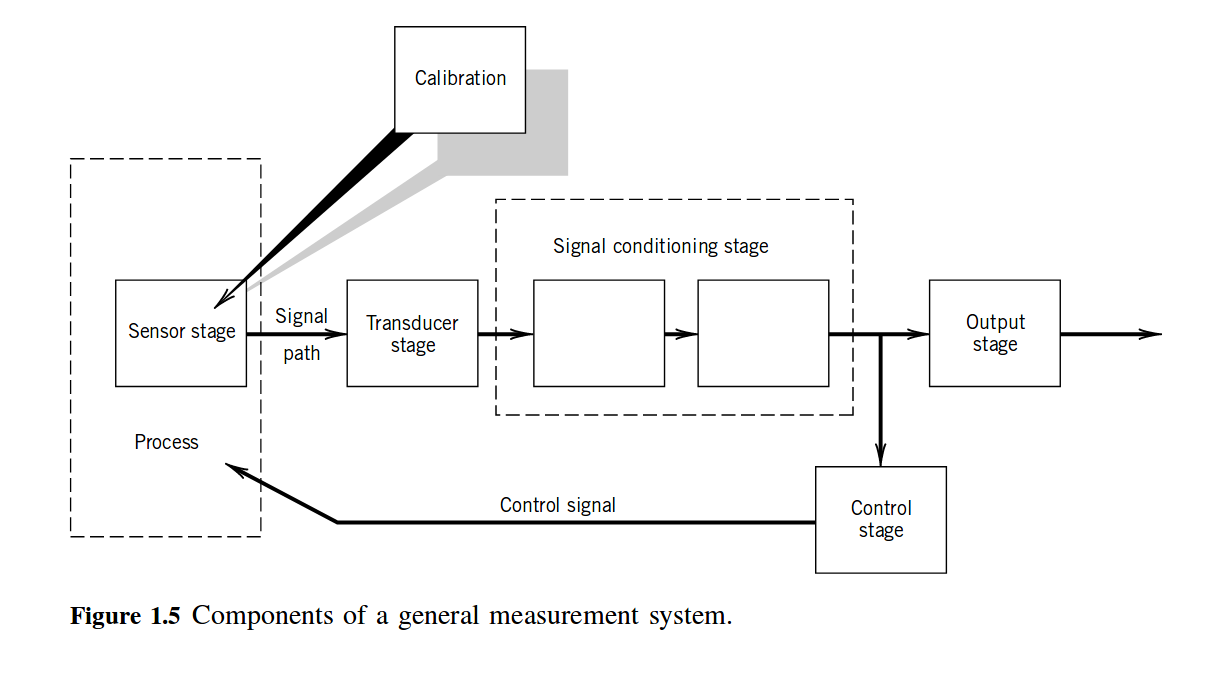
\includegraphics[scale=0.20]{measurement_stages.png}

	\btVFill
	{\tiny Image: Theory and Design of Mech. Meas.}
	
}

% Section I - Frame II:
\frame{  \small
\frametitle{\sectiontitleI}

	Generate ideas as a group. 
	\btVFill

}

% Section I - Frame III:
\frame{  \small
\frametitle{\sectiontitleI}

	(space for more ideas) 
	\btVFill
}

\section{\sectiontitleII}
% Section II - Frame I:
\frame{  \small
\frametitle{\sectiontitleII}

\begin{tabular}{|c|c|c|} \hline
 	Analog \hspace*{10mm}& Digital \hspace*{10mm}& Both? \hspace*{10mm} \\ \hline   
\end{tabular}
 	
 
 \btVFill
}

\section{\sectiontitleIII}

% Section III - Frame I:
\frame{  \small
\frametitle{\sectiontitleIII}

	Thought Exercise: How do we measure distance (aka range)?                                 
 
    \btVFill
}

% Section III - Frame II:
\frame{  \small
\frametitle{\sectiontitleIII}
 

}


\section{\sectiontitleIV}

% Section IV - Frame I:
\frame{  \small
\frametitle{\sectiontitleIV}

	{\bf Thought Exercise:} How do we measure motion?        
	
		\begin{itemize}
		
			\item What variable or quantity is used to describe motion?                         
			\begin{itemize}
				\item
				\item
				\item	
			\end{itemize} \vspace{5mm}
			\item What type of sensor is used to measure this?
			\begin{itemize}
				\item
				\item
				\item	
			\end{itemize}	

		\end{itemize}
	
	\btVFill


}

% Section IV - Frame II:
\frame{  \small
\frametitle{\sectiontitleIV}



}


\end{document}

